\chapter{Compiladores}



\section{Conceptos básicos sobre compiladores}

% --------- CONCEPTO DE COMPILACION


\subsection{Concepto de Compilación}

    \textbf{Compilación}: Conjunto de procesos efectuados para obtener un archivo ejecutable
    a partir de código fuente. \cite{von_hagen_definitive_2006}

% --------- TIPOS DE COMPILADORES

\subsection{Tipos de Compiladores}

    Los siguientes conceptos son fundamentales para introducir la clasificación.
    \begin{itemize}
        \item \textbf{\emph{Host}}: arquitectura de la máquina en la que va a correr el compilador.
        \item \textbf{\emph{Build}}: arquitectura que se usa para generar el compilador.
        \item \textbf{\emph{Target}}: arquitectura en la que deberá correr el ejecutable generado por el
        compilador. 
    \end{itemize}
    
    \begin{table}[t]
        \centering
            \caption{Clasificación de compiladores.}
            \label{tab:TiposCompiladores}
            \begin{tabular}{ | p{0.23\linewidth} | p{0.7\linewidth} | }
                \hline
                \textbf{Tipo de compilador}  & \textbf{Descripción}  \\ \hline
                \textbf{Compilador nativo}  & Compilador que genera  ejecutables para el mismo tipo de sistema en  el cual está operando. (Ídem \emph{build}, \emph{host} y \emph{target})  \\ \hline
                \raggedright \textbf{Compilador “cruzado”}  & Llamado \emph{cross-compiler} en inglés, compilador que corre en una arquitectura específica y genera código para otra distinta. (idem \emph{build} y \emph{host}, distinto \emph{target})   \\ \hline
                \textbf{\emph{Crossback compiler}}    & El sistema en donde corre y el de ejecución de binarios son iguales pero el sistema \emph{host} es distinto. (idem \emph{build} y \emph{target}, distinto \emph{host}).  Se usan para construir un \emph{cross-compiler} que corra en el sistema en el que el compilador corre)  \\ \hline
                \textbf{\emph{Crossed native compiler}}    & El sistema \emph{target} y el \emph{host} son los mismos pero el sistema en donde se construye el compilador es distinto. Usa un \emph{cross-compiler} para construir un compilador nativo en un tercer sistema. (idem \emph{target} y \emph{host}, distinto \emph{build})  \\ \hline
                \raggedright \textbf{Compilador canadiense}    &   El sistema en donde se construye, el \emph{host} y el de destino son todos distintos. Un compilador que construye sobre una arquitectura, corre en otra arquitectura y crea código para una tercera arquitectura. (\emph{build}, \emph{host} y \emph{target} son distintos)   \\ \hline
            \end{tabular}
        \par
    \end{table}

    Así, se presenta la clasificación de los distintos tipos de compiladores (Von Hagen, \cite{von_hagen_definitive_2006}) en la tabla ~\ref{tab:TiposCompiladores}.

    %figure:    h = here // t = top // b = bottom // p = page of float 


% --------- ESTRUCTURA DE COMPILADORES

\subsection{Estructura de un Compilador}

    \label{estructuraCompiladores}

    \begin{figure}[t]
        \begingroup
            \centering
                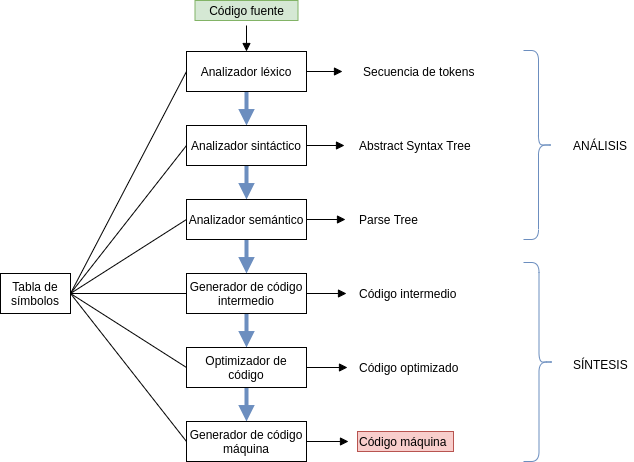
\includegraphics[scale=0.5]{fases_comp}
                \caption{Fases de compilación.}
                \label{fig:fasesComp}
            \par
        \endgroup

    \end{figure}

    Las fases que componen un compilador \cite{aho_compilers:_2007} pueden verse en la Fig. ~\ref{fig:fasesComp}.

\subsubsection{Analizador léxico}

    El analizador léxico, también llamado \emph{scanner} o \emph{lexer}, es aquel que lee la secuencia de caracteres del código fuente y los agrupa en
    otras secuencias llamadas \textbf{lexemas}. Por cada lexema, el \emph{scanner} genera un \emph{token} de la forma:
    La Fig. ~\ref{fig:fasesEjemplo} muestra las entradas y salidas de la fase en la parte superior.

    \begin{equation}
    \label{eq:1}
    <nombre\text{-}token, valor\text{-}atributo>
    \end{equation}
    Siendo, 
    \begin{itemize}
        \item \textbf{nombre-token}: símbolos abstractos usados durante el análisis sintáctico.
        \item \textbf{valor-atributo}: puntero a una entrada en la tablas de símbolos.
    \end{itemize}

    \paragraph*{Tabla de símbolos}

    El compilador guarda los nombres de variables o nombres de funciones (que aparecen en el
    código fuente) en la \textbf{tabla de símbolos}. También, almacena atributos 
    varios de dicha variable,
    por ejemplo: tipo, \emph{scope}, argumentos, tipo de pasaje de argumentos, 
    tipo de retorno, etc.
    Luego, se realiza un mapeo de \emph{tokens} con sus respectivos nombres de la tabla.

\subsubsection{Analizador sintáctico}

    El analizador sintáctico, también llamado \emph{parser}, utiliza el primer componente de cada \emph{token} ($nombre\text{-}token$ en ecuación ~\ref{eq:1}) para crear una representación en
    forma de árbol que muestre la estructura de los \emph{tokens}. Se genera un  \textbf{árbol sintáctico}. La Fig. ~\ref{fig:fasesEjemplo} refleja un esquema de esta fase en la parte superior.


\subsubsection{Analizador semántico}

    El analizador semántico emplea el árbol sintáctico y la tabla de símbolos (creada por el \emph{scanner}) para revisar la
    consistencia semántica del código fuente con respecto a la definición del lenguaje. También se realizan conversiones de un tipo de dato a otro (llamadas coerciones).
    Ver Fig. ~\ref{fig:fasesEjemplo} en la fase correspondiente.


\subsubsection{Generador de código intermedio}

    El generador intermedio tiene como meta producir código de tipo intermedio para obtener un lenguaje flexible y optimizable para la
    parte \emph{backend} del compilador. Observar dentro de la Fig. ~\ref{fig:fasesEjemplo} para una ilustración de la fase.

    El código intermedio puede tener muchas formas distintas (dependiendo de cada compilador).

\paragraph*{Propiedades de todo código intermedio}

Todo código intermedio debe cumplir las propiedades de:

    \begin{enumerate*}[label=\itshape\alph*\upshape)]
        \item ser fácil de generar;
        \item ser fácil de traducir a lenguaje máquina
    \end{enumerate*}

\paragraph*{Código de tres direcciones}

    Es una forma de código intermedio que consiste en una secuencia de instrucciones
    cuasi-\emph{assembler} con tres operandos por cada instrucción (cómo máximo). Cada
    operando puede actuar como un registro.

    Algunas características de este tipo de código son:

    \begin{itemize}
        \item Las instrucciones deben tener como máximo un \textbf{único operador} (órden de
        operaciones)
        \item El compilador debe generar un \textbf{nombre temporal} para guardar el valor retornado
        por la instrucción de tres direcciones (variables temporales tienen nombre).
    \end{itemize}


\subsubsection{Optimizador de código intermedio}

    El optimizador de código intermedio realiza mejoras sobre  dicho código para obtener un “mejor código” como salida de
    cada sucesiva optimización. Se presenta también una ilustración en la parte inferior de la Fig. ~\ref{fig:fasesEjemplo}.

    \begin{center}
        Mejor código = más rápido, más corto o de menor consumo de potencia.
    \end{center}

\subsubsection{Generador de código final}

    El generador de código final utiliza el código optimizado para generar el código final deseado.
    Si el lenguaje final es código máquina, se eligen los registros o lugares de memoria para
    cada variable usada en el programa. 
    En este trabajo, el código final buscado es código máquina. Por ello, se empleará el término "generador de código máquina".
    En este caso, se traducen instrucciones inmediatas a secuencias de instrucciones máquina.
    La parte inferior de la Fig. ~\ref{fig:fasesEjemplo} muestra una ilustración sobre esta fase.

    \begin{figure}[p]
        \begingroup
            \centering
                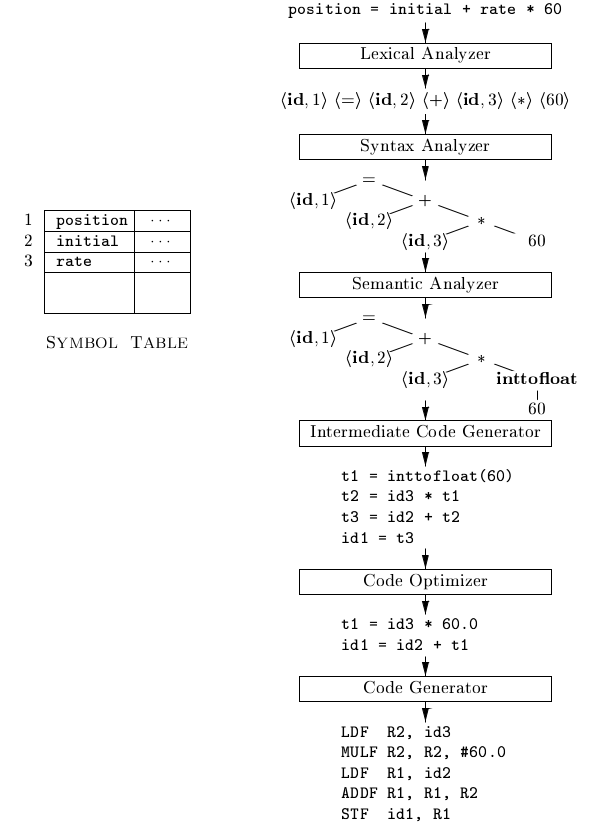
\includegraphics[width=0.8\textwidth,height=0.8\textheight,keepaspectratio]{ejemplo_fasescomp}
                \caption{Ejemplo completo de fases de compilación.\cite{aho_compilers:_2007}}
                \label{fig:fasesEjemplo}
            \par
        \endgroup
    \end{figure}
